\documentclass[xcolor=dvipsnames]{beamer}
\usepackage{amsmath, amsfonts, epsfig, xspace}
\usepackage{algorithm,algorithmic}
\usepackage{pstricks,pst-node}
\usepackage{multimedia}
\usepackage[normal,tight,center]{subfigure}



%\usetheme{Luebeck}
\usetheme[secheader]{Madrid}


\definecolor{color1}{RGB}{56,115,178}
\definecolor{color2}{RGB}{115,115,115}
%\usepackage[pdftex=true,hyperindex=true,colorlinks=true,linkcolor=color2]{hyperref}

\usecolortheme[named=color1]{structure}
\usepackage{graphicx}
\usepackage{thumbpdf}
\usepackage{ucs}
\usepackage[utf8]{inputenc}
\usepackage{pgf,pgfarrows,pgfnodes,pgfautomata,pgfheaps,pgfshade}
\usepackage{verbatim}
\usepackage{fancybox} %pour la forme des box
\usepackage{pstricks}%pour les organigrammes
\usepackage{algorithm,algorithmic}%pour les algorithmes
\usepackage[francais]{babel}

%\usepackage[math]{kurier}
%\usepackage[T1]{fontenc}
\usepackage[condensed,math]{iwona}

\title[Cloud Computing]{Gestion de la consommation d’énergie dans\\ les Clouds Computing}
\author{Pr\'esent\'e par :\\ \textbf{\textsc{YAGOUBI Djamel Edine}} }
%\institute{}
\logo{%
    
\includegraphics[width=1cm,height=1cm,keepaspectratio]{logo-univ2.png}~%
}
\date{{ 18 Juin 2014}}


\begin{document}

     %%   La page de garde 
\begin{frame}
\begin{center}
\scalebox{9}{
\includegraphics[width=1cm,height=1cm,keepaspectratio]{logo-univ.png}}
\end{center}
\titlepage
{\scriptsize Encadreur:\textbf{ Mr BELALEM Ghalem}
                         \\ Co-Encadreur:\textbf{ Mlle DAD Djouhra }}                         
\end{frame}



\begin{frame}
\frametitle{Sommaire}
\tableofcontents[hideothersubsections]
\end{frame}



%\AtBeginSection[]
%{
%  \begin{frame}
%  \frametitle{Sommaire}
%  \tableofcontents[currentsection, hideothersubsections,
%pausesubsections]
%  \end{frame} 
%}

% Problématique
\section{Introduction}
\subsection{Contexte}

\begin{frame}
\frametitle{Contexte}
\begin{columns}
\begin{column}{0.45\textwidth}

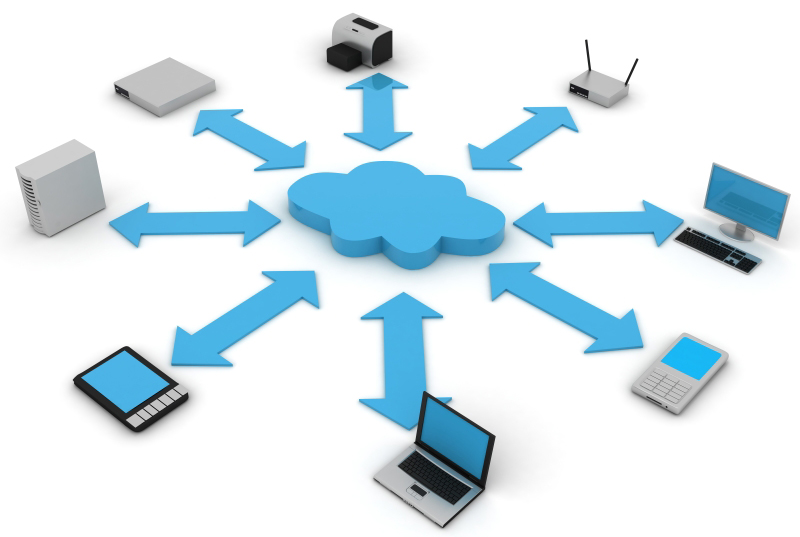
\includegraphics[scale=0.2]{cloud-computing.jpg}
\begin{block}{}
\begin{minipage}{\textwidth}
\begin{center}
Le Cloud Computing 
\end{center}

\end{minipage}
\end{block}

\end{column}
\begin{column}{0.5\textwidth}
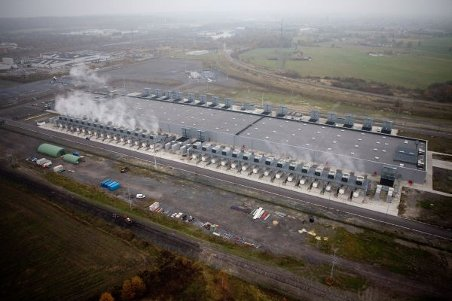
\includegraphics[scale=0.38]{dt.jpg}
\begin{block}{}
\begin{minipage}{\textwidth}
\begin{center}
Les Data Centers
\end{center}

\end{minipage}
\end{block}
\end{column}

\end{columns}


\end{frame}
\subsection{Problématique}

\begin{frame}
\frametitle{Le poids des Data Centers dans la consommation électrique}
\begin{columns}
\begin{column}{0.55\textwidth}
\begin{block}{}
\begin{itemize}
\item \textbf{1,5\%} de la consommation électrique mondiale d’environ \textbf{8000 MWh};
\item \textbf{2\%} des émissions mondiales de \textbf{CO²};
\item Certains Data Centers consomment plus qu'une ville de \textbf{100.000 habitants};
\item La puissance électrique des cloud data centers dans le monde correspond à la capacité de production de \textbf{30} centrales nucléaires;
\end{itemize}
\end{block}
\end{column}
\begin{column}{0.40\textwidth}
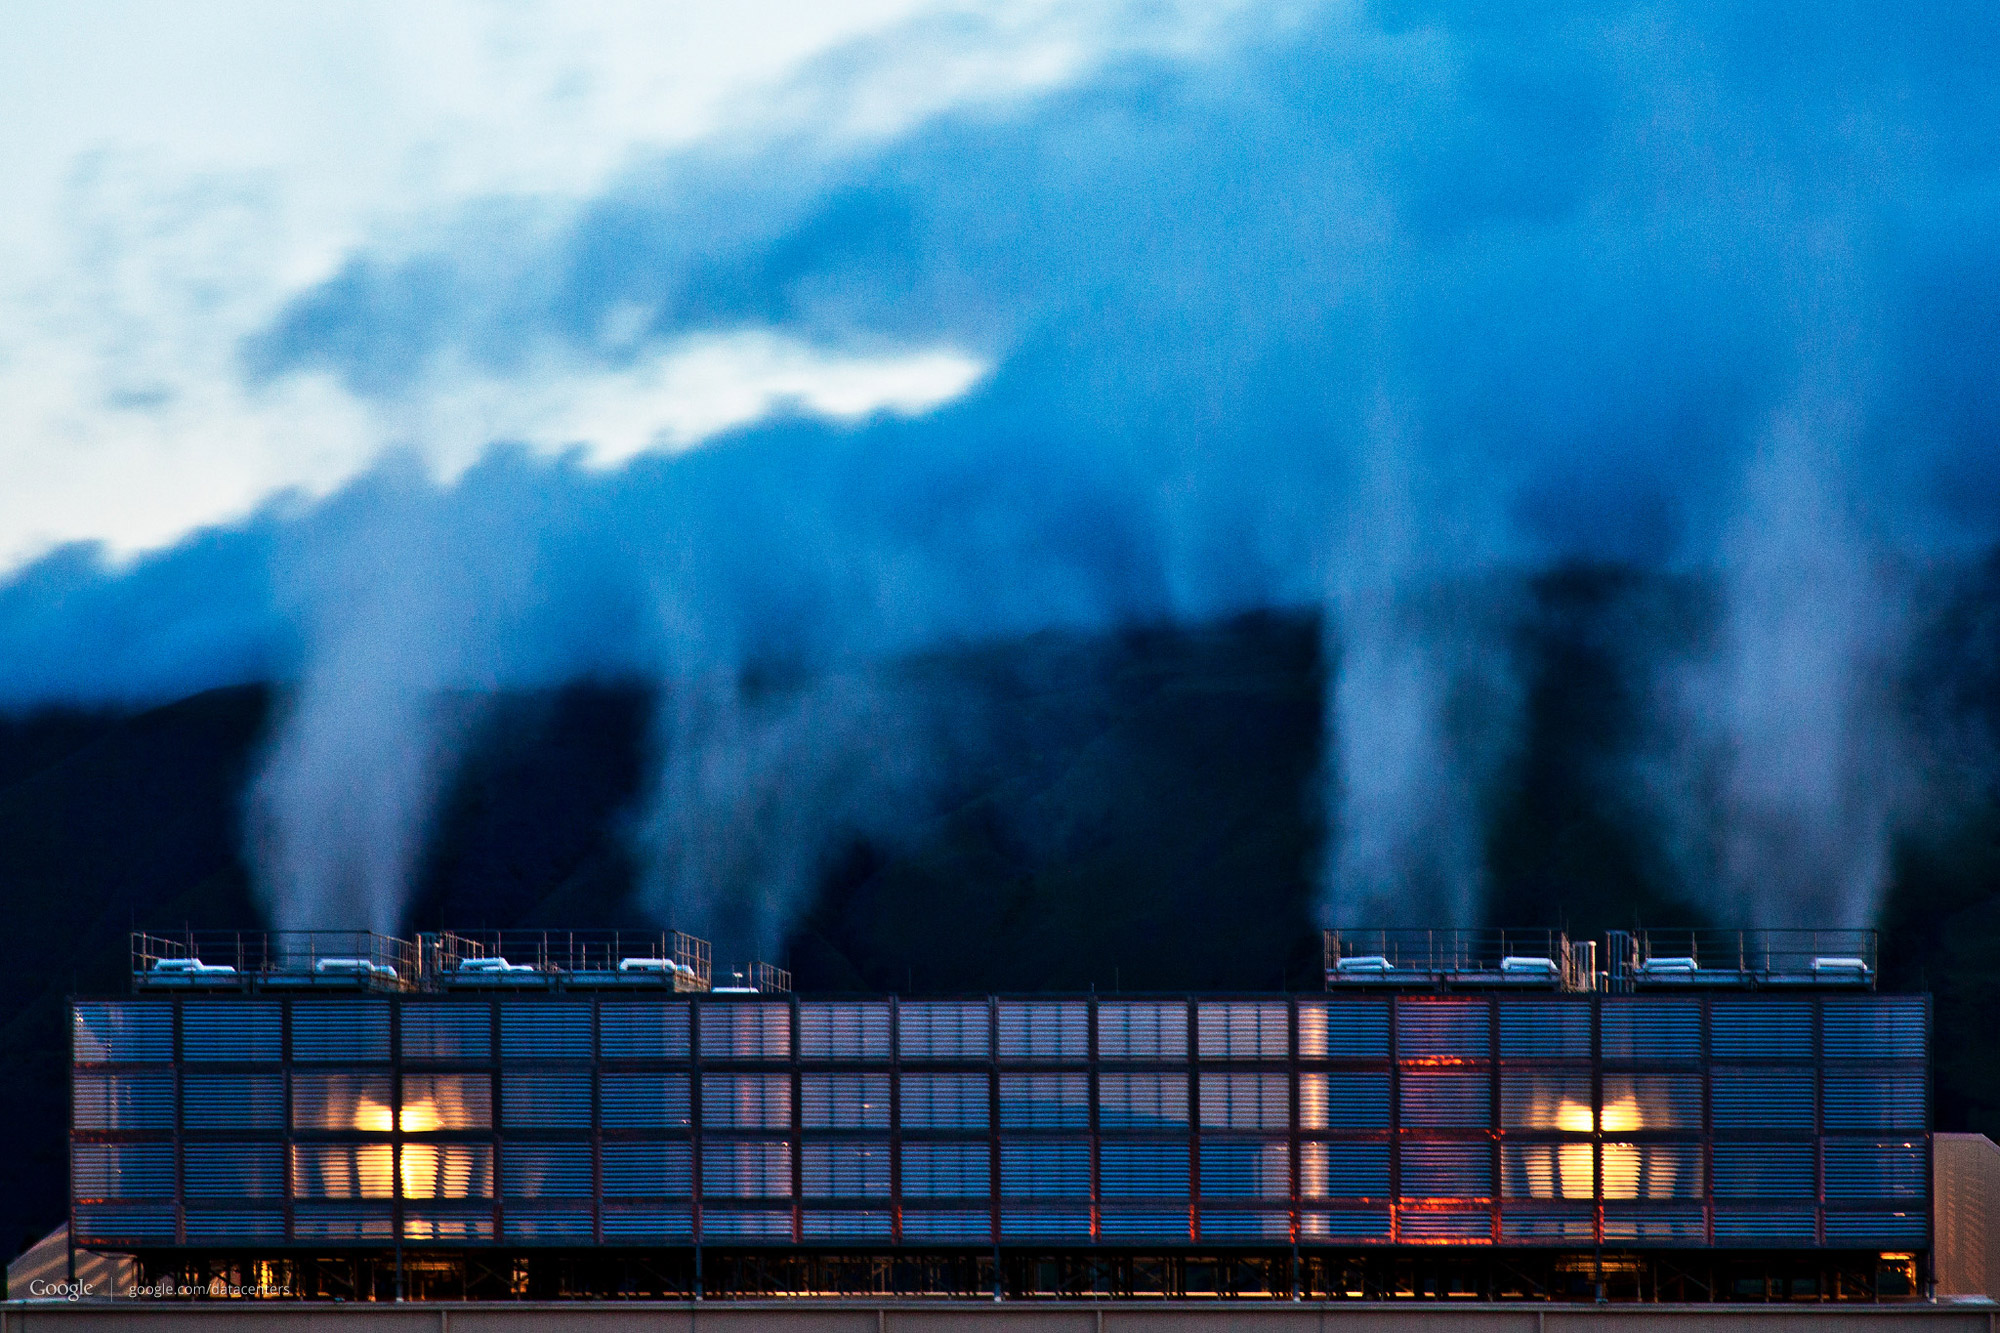
\includegraphics[scale=0.072]{datacentre2.jpg}
\end{column}

\end{columns}
\end{frame}


\begin{frame}
\frametitle{Pourquoi les data centers consomment autant d'énergie ?}
\begin{columns}
\begin{column}{0.55\textwidth}
\begin{block}{}
\begin{itemize}
\item les serveurs de stockage ne peuvent pratiquement jamais être arrêtés.
\end{itemize}
\end{block}
\begin{block}{}
\begin{itemize}
\item Le bon fonctionnement des serveurs est assuré par des systèmes de climatisation très énergivores.
\end{itemize}
\end{block}
\end{column}
\begin{column}{0.40\textwidth}
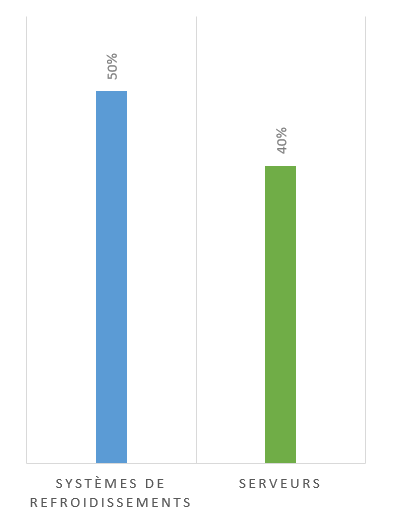
\includegraphics[scale=0.5]{conso.png}
\end{column}
\end{columns}
\end{frame}


\begin{frame}
\frametitle{Consommations d'énergie au niveau des serveur}


\begin{columns}
\begin{column}{0.70\textwidth}
\begin{block}{}
\begin{minipage}{\textwidth}
Les serveurs consomment environ \textbf{40\%} de la consommation d’énergie totale des Data Centres.
\end{minipage}
\end{block}
\begin{block}{}
\begin{minipage}{\textwidth}
Un serveur qui n’utilise que \textbf{20\%} de sa capacité de calcul utilise déjà \textbf{70\%} de sa puissance électrique maximale.
\end{minipage}
\end{block}
\begin{block}{}
\begin{minipage}{\textwidth}
L'énergie utilisée pour faire fonctionner ces serveurs non utilisés pourraient compenser les émissions de \textbf{CO²} de \textbf{6,5} millions de véhicules \cite{ref1}. 
\end{minipage}
\end{block}
\end{column}
\begin{column}{0.25\textwidth}
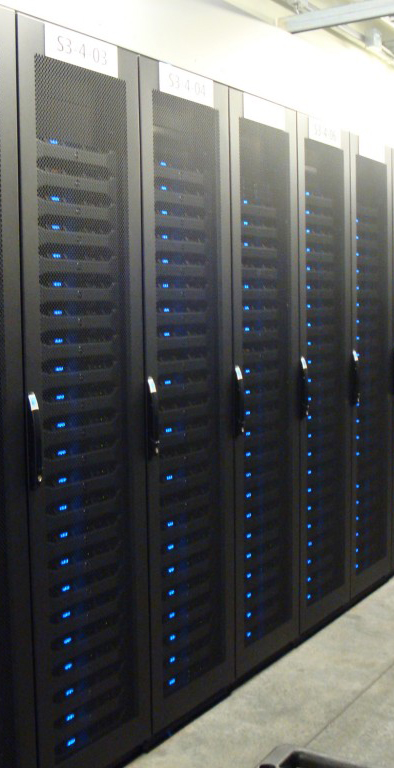
\includegraphics[scale=0.2]{server.jpg}
\end{column}

\end{columns}

\end{frame}



%Objectif
\subsection{Objectif}

\begin{frame}
\frametitle{Objectif}

\begin{center}
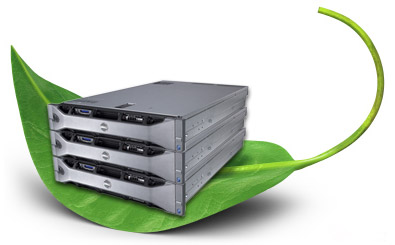
\includegraphics[scale=0.5]{green-server.jpg}
\end{center}
\begin{block}{}
\begin{center}
comment réduire la consommation d'énergie des serveurs ?
\end{center}
\end{block}

\end{frame}



%Approche Proposée
\section{Conception et Implémentation}
\subsection{Migration}
\begin{frame}
\begin{columns}
\begin{column}{0.50\textwidth}
%\frametitle{Migration}
\begin{center}
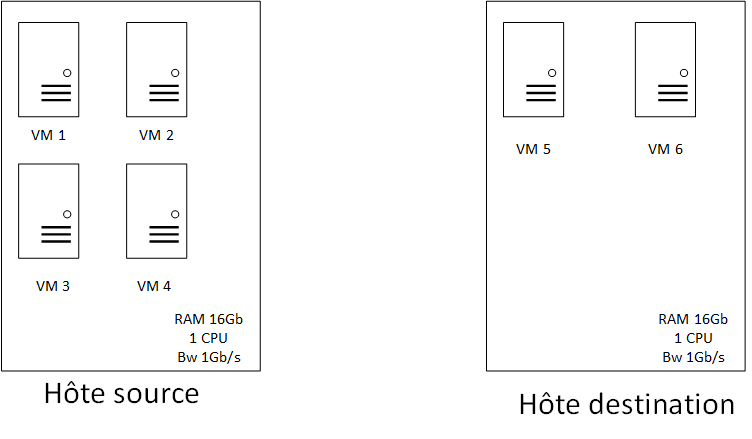
\includegraphics[scale=0.3]{migration.png}
\end{center}

%\end{column}

%\begin{column}{0.50\textwidth}
\begin{center}
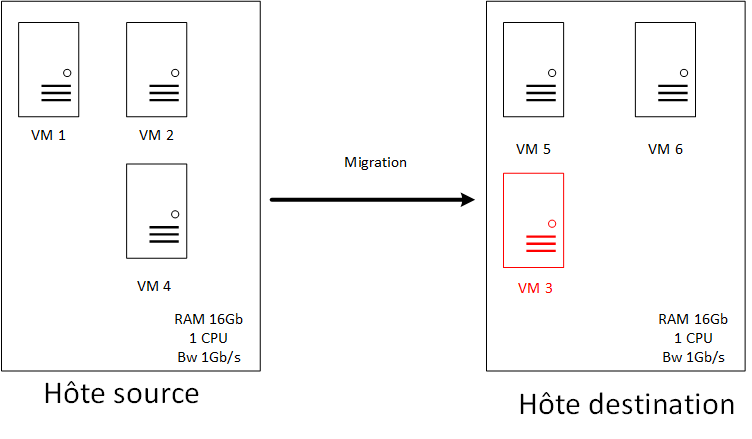
\includegraphics[scale=0.3]{migration2.png}
\end{center}
\end{column}
\end{columns}
\end{frame}




\begin{frame}

\begin{block}{}
\begin{center}
\Huge La minimisation des migrations des machines virtuelles
\end{center}
\end{block}

\end{frame}



\subsection{Les étapes de migration}
\begin{frame}
\frametitle{Les étapes de migration}
\begin{columns}
\begin{column}{0.40\textwidth}
\begin{center}
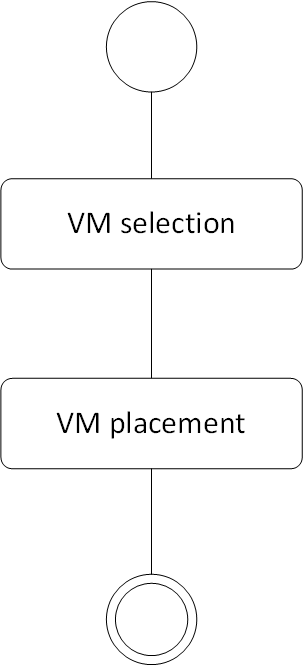
\includegraphics[scale=0.38]{DAM.png}
\end{center}
\end{column}
\begin{column}{0.55\textwidth}
\begin{block}{}
\begin{minipage}{\textwidth}
Quelle VM doit-on choisir pour  faire une migration?
\end{minipage}
\end{block}

\begin{block}{}
\begin{minipage}{\textwidth}

Quel  est le nouvel emplacement de la VM?
\end{minipage}
\end{block}
\end{column}
\end{columns}

\end{frame}
\subsection{Sélection des VMs}
\begin{frame}
\frametitle{Sélection des VMs}
\begin{center}
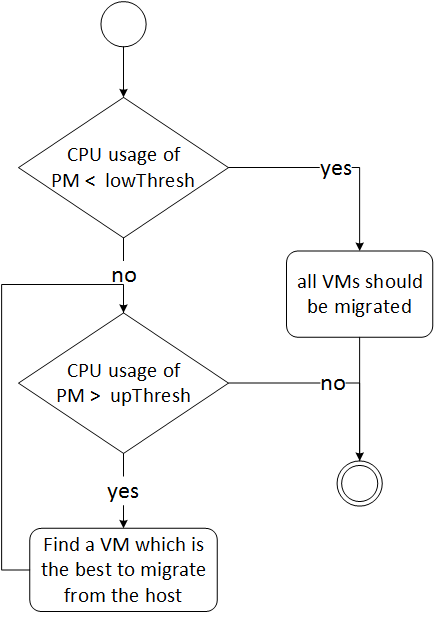
\includegraphics[scale=0.4]{smm.png}
\end{center}
\end{frame}

\subsection{Placement des VMs}
\begin{frame}
\frametitle{Placement des VMs}
\begin{center}
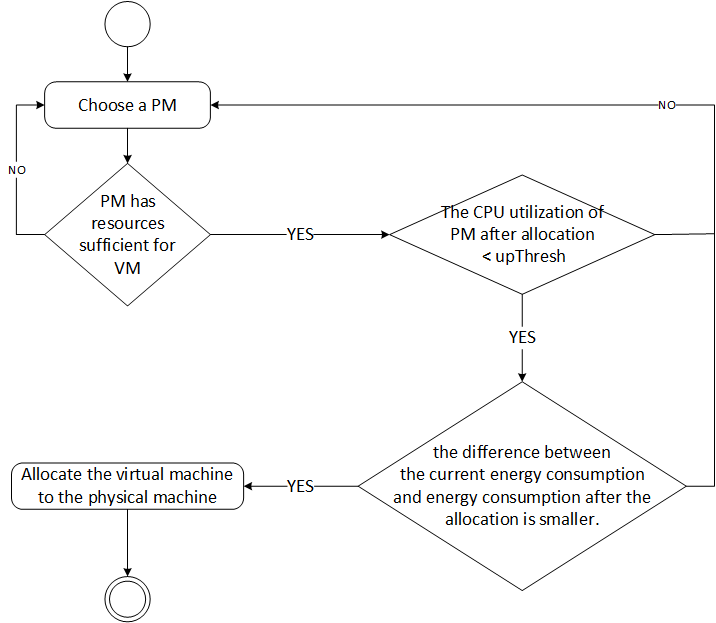
\includegraphics[scale=0.42]{8.png}
\end{center}
\end{frame}

\subsection{Intégration}

\begin{frame}
\begin{block}{}
\begin{center}

\Huge L'implémentation d'algorithmes dans le simulateur cloudsim
\end{center}
\end{block}
\end{frame}

\begin{frame}
\frametitle{ Diagramme de Classes de CloudSim}
\begin{center}
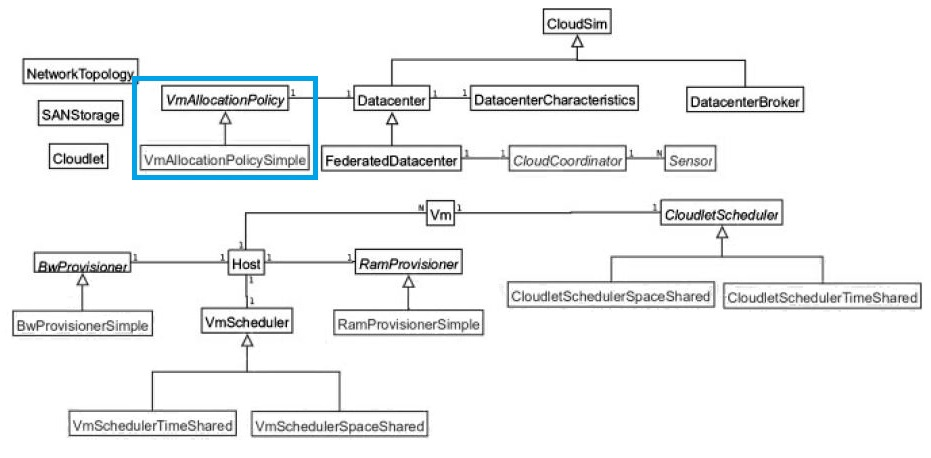
\includegraphics[scale=0.48]{cloudsimclass.JPG}
\end{center}
\end{frame}


\begin{frame}
\frametitle{ Diagramme de Classes de CloudSim}
\begin{center}
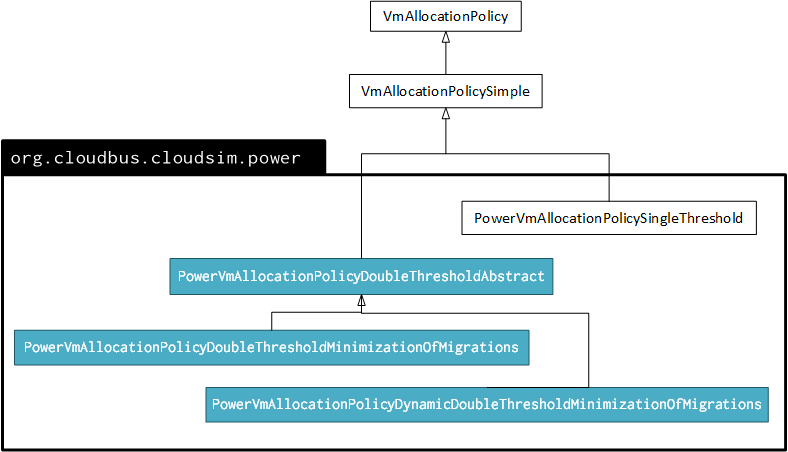
\includegraphics[scale=0.50]{CloudSimclass.png}
\end{center}
\end{frame}

\section{Résultats}
\begin{frame}
\begin{block}{}
\begin{center}

\Huge Résultats
\end{center}
\end{block}

%\begin{block}{}
\begin{center}

\begin{center}
{\footnotesize   \begin{tabular}{|p{6cm}|c|}
\hline
      \centering     Paramètres &  Valeurs\\
\hline
     \centering       Nombre de Data Center &  1\\
\hline
      \centering      Nombre de hôtes &  100\\
\hline
      \centering      Nombre de processeurs de chaque hôte &  1\\
\hline
      \centering      Vitesse de processeur de chaque hôte (MIPS)&  1000,2000 ou 3000\\
\hline

      \centering    RAM du hôte &  8GB\\
\hline
      \centering    Stockage du hôte &  1TB\\
\hline
      \centering      Nombre de VMs &  29 à 290\\
\hline
      \centering      Nombre de processeur de chaque VM &  1\\
\hline
      \centering    Vitesse de processeur de chaque VM (MIPS) &  250, 500, 750 ou 1000\\
\hline

      \centering    RAM de chaque VM &  128MB\\
\hline
     \centering    Stockage du VM &  1GB\\
\hline

\end{tabular}}
%\captionof{table}{Comparaison entre la consommation d’énergie des quatre approches}
\end{center}

%Dans cette simulation, nous avons créé un Data Center contenant 100 hôtes hétérogènes, Chaque hôte posséde 1 processeur avec une vitesse variante en MIPS (1000, 2000 ou 3000), 8GB de mémoire, 1TB de stockage. Le Broker fait varier un nombre de VMs hétérogène de 29 à 290 pour chaque VM a 1 processeur avec une vitesse variante en MIPS (250, 500, 750 ou 1000), 128MB de mémoire, 1GB de stockage.
\end{center}
%\end{block}
\end{frame}


\begin{frame}
\frametitle{Consommation d’énergie}
\begin{center}
{\tiny  \begin{tabular}{|p{3cm}|c|c|c|c|c|c|c|c|c|c|}
\hline
      \centering     Nombre de VMs &  29& 58& 87& 116& 145& 174& 203& 232& 261& 290\\
\hline
     \centering       Approche sans migration &  5.21& 10.83& 16.61& 22.45& 27.57& 33.69& 38.65& 44.15& 50.22& 60.55\\
\hline
      \centering      Single Threshold &  4.69& 9.30& 13.78& 18.39& 22.80& 27.78& 33.21& 38.14& 43.97& 49.98\\
\hline
      \centering      \color{red}Fixed Double Threshold &  3.90& 7.86& 11.73& 15.76& 19.53& 23.66& 27.62& 32.06& 36.38& 40.93\\
\hline
      \centering    \color{red} Dynamic Double Threshold &  3.67& 7.19& 10.56& 13.89& 17.62& 20.63& 24.61& 27.97& 31.91& 36.26\\
\hline
\end{tabular}}
%\captionof{table}{Comparaison entre la consommation d’énergie des quatre approches}
\end{center}



\begin{center}
{\tiny   \begin{tabular}{|p{3.5cm}|c|}
\hline
      \centering      Nom de l’approche &  Gain\\
\hline
     \centering       Approche sans migration et Dynamic Double Threshold &  36,21\%\\
\hline
      \centering      Single Threshold et Dynamic Double Threshold&  24,81\%\\
\hline
      \centering      Fixed Double Threshold et Dynamic Double Threshold&  10,61\%\\
\hline
\end{tabular}}

\end{center}
\end{frame}

\begin{frame}
\frametitle{Consommation d’énergie}
\begin{center}
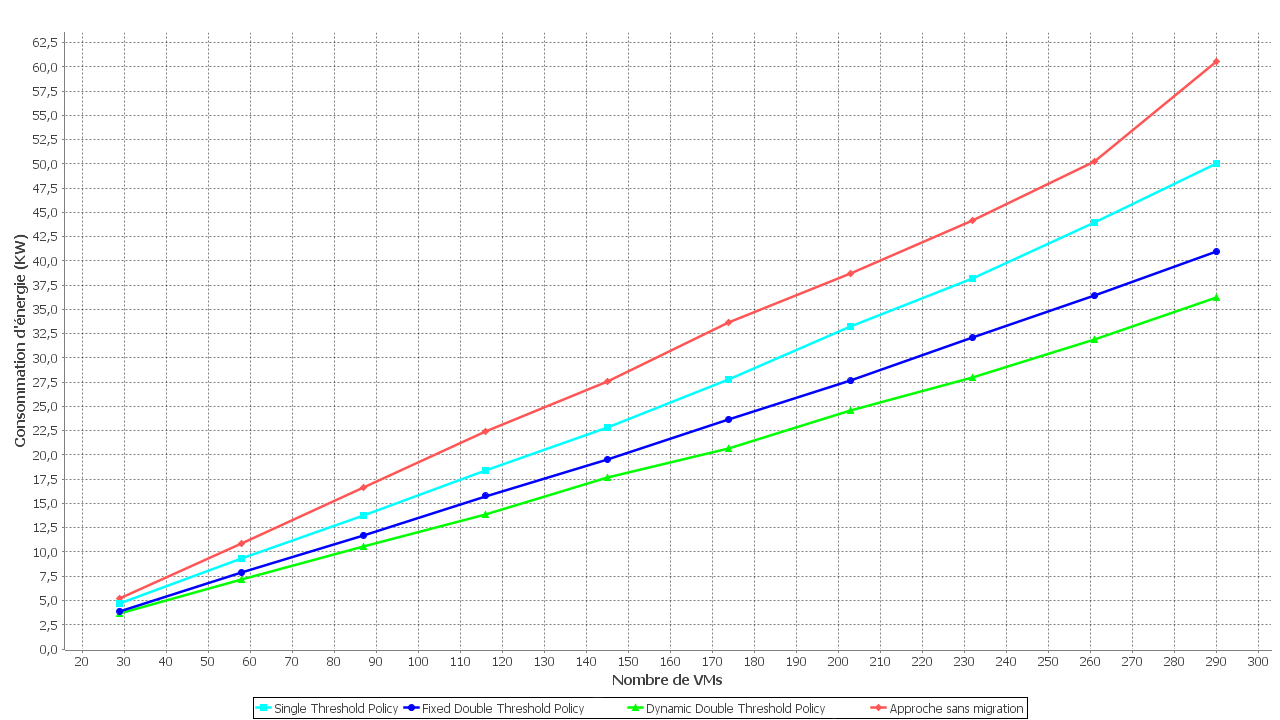
\includegraphics[scale=0.25]{sh1.png}
\end{center}
\end{frame}



\begin{frame}
\frametitle{Nombre de migrations}
\begin{center}
{\tiny  \begin{tabular}{|p{2cm}|c|c|c|c|c|c|c|c|c|c|}
\hline
      \centering     Nombre de VMs &  29& 58& 87& 116& 145& 174& 203& 232& 261& 290\\
\hline
      \centering      Single Threshold &  4589& 10885& 16807& 22970& 29323& 35502& 41896& 48240& 54692& 61072\\
\hline
      \centering      \color{red}Fixed Double Threshold &  2060& 5638& 10049& 15038& 18630& 25452& 29861& 34003& 40886& 44736\\
\hline
      \centering     \color{red}Dynamic Double Threshold &  415& 1446& 1976& 2674& 3715& 4363& 5291& 6714& 7448& 9346\\
\hline
\end{tabular}}
%\captionof{table}{Comparaison entre la consommation d’énergie des quatre approches}
\end{center}



\begin{center}
{\tiny   \begin{tabular}{|p{3.5cm}|c|}
\hline
      \centering      Nom de l’approche &  Gain\\
\hline
      \centering      Single Threshold et Dynamic Double Threshold&  87,38\%\\
\hline
      \centering      Fixed Double Threshold et Dynamic Double Threshold&  80,31\%\\
\hline
\end{tabular}}

\end{center}
\end{frame}

\begin{frame}
\frametitle{Nombre de migrations}
\begin{center}
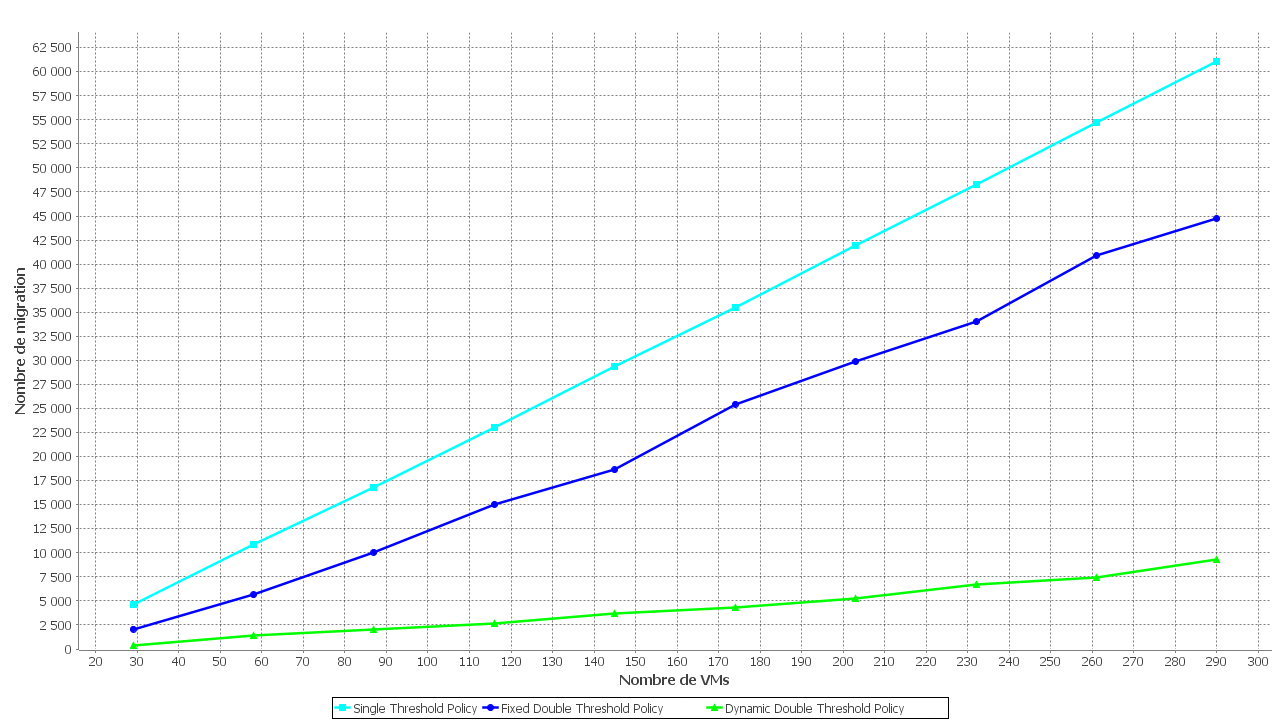
\includegraphics[scale=0.25]{sh2.png}
\end{center}
\end{frame}



\begin{frame}
\frametitle{Violation de SLA}
\begin{center}
{\tiny  \begin{tabular}{|p{2.5cm}|c|c|c|c|c|c|c|c|c|c|}
\hline
      \centering     Nombre de VMs &  29& 58& 87& 116& 145& 174& 203& 232& 261& 290\\
\hline
      \centering      Single Threshold &  4786& 12420& 20010& 27810& 36461& 44241& 52839& 61543& 70830& 79590\\
\hline
      \centering     \color{red}Fixed Double Threshold &  3023& 8827& 16125& 23449& 30604& 40439& 48878& 55547& 67278& 75000\\
\hline
      \centering     \color{red}Dynamic Double Threshold &  993& 3840& 6402& 8112& 12821& 15182& 17325& 22882& 26316& 29488\\
\hline
\end{tabular}}
%\captionof{table}{Comparaison entre la consommation d’énergie des quatre approches}
\end{center}



\begin{center}
{\tiny   \begin{tabular}{|p{3.5cm}|c|}
\hline
      \centering      Nom de l’approche&  Gain\\
\hline
      \centering      Single Threshold et Dynamic Double Threshold&  67,35\%\\
\hline
      \centering      Fixed Double Threshold et Dynamic Double Threshold&  61,48\%\\
\hline
\end{tabular}}

\end{center}
\end{frame}

\begin{frame}
\frametitle{Violation de SLA}
\begin{center}
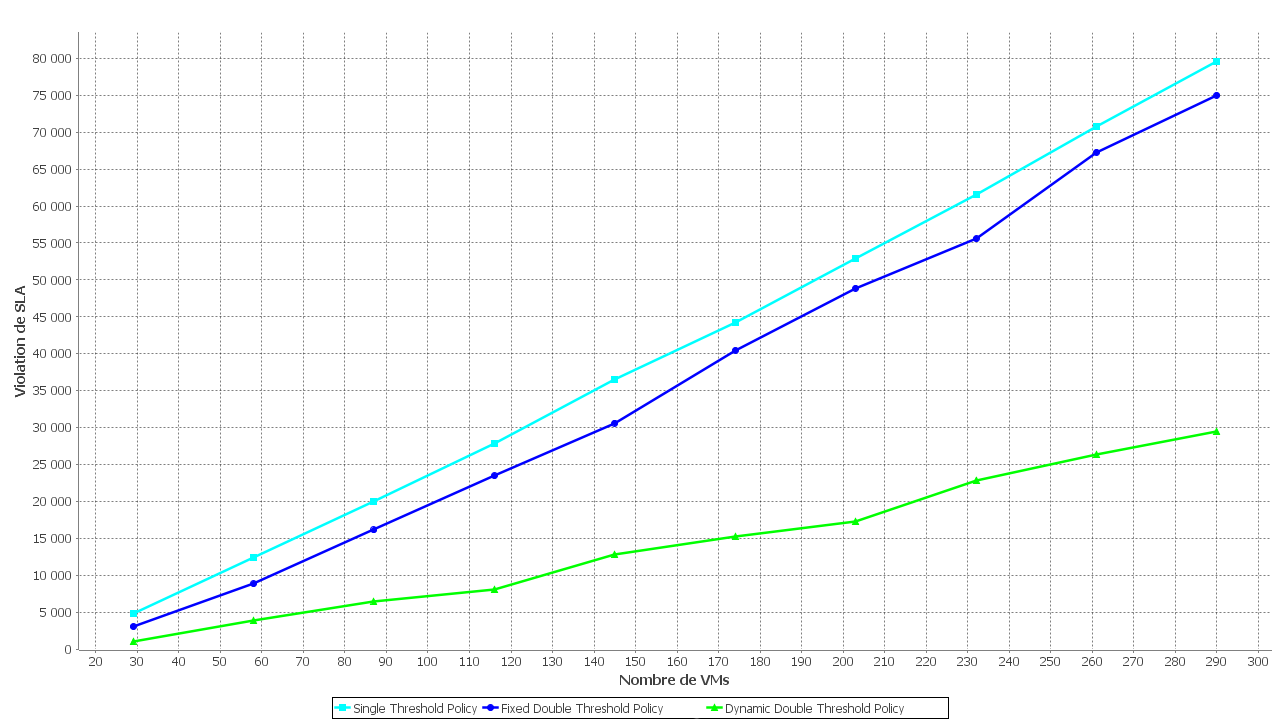
\includegraphics[scale=0.25]{sh3.png}
\end{center}
\end{frame}


\section{Conclusion et Perspectives}


\begin{frame}
%\frametitle{Conclusion}
\begin{center}
\begin{block}{Conclusion}
Nous avons proposé deux approches qui permettent:
\begin{itemize}
\item  La minimisation de la consommation d'énergie par rapport aux approches classiques.
\item La réduction du nombre de migrations des VMs
\item La réduction du nombre de violations de SLA
\end{itemize}
\vspace{0.5cm}
Les résultats obtenus sont très encourageant qui dénotent la puissance de nos propositions.
\end{block}
\end{center}
\end{frame}


\begin{frame}
\begin{center}
\begin{block}{Perspectives}
\begin{itemize}
\item En plus de l'utilisation du processeur, prendre en considération   plusieurs ressources au niveau de la phase de migration tels que : la capacité de la RAM, la capacité de stockage et la bande passante.
\item Ajouter un seuil de température afin de limiter la chaleur dégagée des machines physiques et de minimiser l'énergie consommée des serveurs et des systèmes de refroidissement.
\item Implémenter les deux approches proposées dans un environnement de Cloud réel.
\item Étudier l'influence des systèmes de climatisation des data center sur leur efficacités et leur performances.



\end{itemize}
\end{block}
\end{center}
\end{frame}





\begin{frame} 
\begin{block}{}
\begin{center}
\textbf{
{\Huge Merci de votre attention !}}
\end{center}
\end{block}
\vspace{3cm}
{\tiny \setbeamertemplate{bibliography item}[text] 
\begin{thebibliography}{99} 

\bibitem[1]{ref1} Powering the cloud, groupe ABB, \url{http://www.abb.com/product/ap/db0003db004052/e950c90f13518ffbc125788f0030bda0.aspx} consilté le 16/06/2014.

\end{thebibliography} }
\end{frame} 

\end{document}



